\documentclass{beamer}

% This file is a solution template for:

% - Giving a talk on some subject.
% - The talk is between 15min and 45min long.
% - Style is ornate.



% Copyright 2004 by Till Tantau <tantau@users.sourceforge.net>.
%
% In principle, this file can be redistributed and/or modified under
% the terms of the GNU Public License, version 2.
%
% However, this file is supposed to be a template to be modified
% for your own needs. For this reason, if you use this file as a
% template and not specifically distribute it as part of a another
% package/program, I grant the extra permission to freely copy and
% modify this file as you see fit and even to delete this copyright
% notice. 


\mode<presentation>
{
  \usetheme{Darmstadt}
}


\usepackage[english]{babel}
\usepackage[latin1]{inputenc}

\title{Worst-Case Execution Time Analysis}

\author{Ryan Fox}

\institute
{
  Department of Electrical and Computer Engineering\\
  University of Waterloo
}

\date{\today}

\AtBeginSubsection[]
{
  \begin{frame}<beamer>{Outline}
    \tableofcontents[currentsection,currentsubsection]
  \end{frame}
}

\begin{document}

\begin{frame}
  \titlepage
\end{frame}

\begin{frame}{Outline}
  \tableofcontents[pausesections]
\end{frame}

\section{Introduction}
\subsection{Definitions}

\begin{frame}{WCET}
  \begin{itemize}
    \item $WCET_A$ -- Actual Worst Case Execution Time
    \item $WCET_D$ -- Derived Worst Case Execution Time
  \end{itemize}
\end{frame}

\begin{frame}{Safety}
  Is $WCET_D \geq WCET_A$ ?
  \begin{itemize}
    \item WCET Bound
      \begin{itemize}
        \item $WCET_A \in (0, WCET_D]$
        \item Safe
      \end{itemize}      
      \pause
    \item WCET Estimate
      \begin{itemize}
        \item Maximum value of all sampled WCETs
        \item Does not consider all possible cases
        \item Not safe          
      \end{itemize}      
  \end{itemize}
\end{frame}

\begin{frame}{Precision}
  \begin{itemize}
    \item Are the bounds or estimates close to the actual values? \\
      \pause
    \item Less Precision
      \begin{itemize}
      \item[$\Rightarrow$] More idle time
        \pause
      \item[$\Rightarrow$] Harder to schedule
      \end{itemize}
  \end{itemize}
\end{frame}

\subsection{Assumptions}

\begin{frame}{Assumptions}
  \pause
  \begin{itemize}
    \item Hard Real-Time System
    \item Execution does not continue indefinitely
    \item Loops and recursion are explicitly bounded \pause
    \item No dynamic jumps
      \begin{itemize}
        \item Function pointers
        \item \texttt{switch} statements
      \end{itemize}
      \pause
    \item No interruptions
  \end{itemize}
\end{frame}

\section{Static Analysis}
\subsection{Frontend}
\begin{frame}{Frontend}
  \begin{columns}
    \begin{column}{0.6\textwidth}
      \begin{itemize}
        \item<1-> Input:
          \begin{itemize}
            \item Source code; or
            \item Machine code; and maybe
            \item User annotations
          \end{itemize}
        \item<2-> Output:
          \begin{itemize}
            \item Call Graph
            \item Control-Flow Graph
            \item Other Information
              \begin{itemize}
              \item Ranges for input data
              \item Iteration/Recursion bounds
              \end{itemize}
          \end{itemize}
      \end{itemize}
    \end{column}
    \begin{column}{0.4\textwidth}
      \begin{center}
        \begin{itemize}
          \item<1->[] 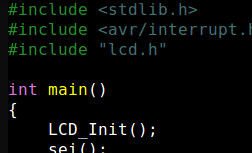
\includegraphics[scale=0.3]{code.png}
          \item<2->[] 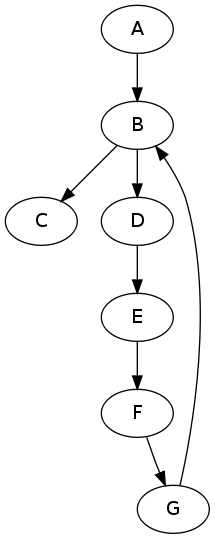
\includegraphics[scale=0.2]{controlflow.png}
        \end{itemize}
      \end{center}      
    \end{column}
  \end{columns}
\end{frame}

\subsection{Control-Flow Analysis}
\begin{frame}{Control-Flow Analysis}
  \begin{columns}
    \begin{column}{0.63\textwidth}
      \begin{itemize}
        \item Finds all possible paths of execution
        \item Attempts to eliminate infeasible paths to improve precission
          \begin{itemize}
            \item \texttt{if (a > 20 \&\& a == (b \% 10))}
          \end{itemize}
        \item Determines bounds of iteration and recursion
        \item<2-> Challenges:
          \begin{itemize}
            \item Dynamic jumps
            \item Pipelining
            \item Out-of-order execution
          \end{itemize}
      \end{itemize}
    \end{column}
    \begin{column}{0.37\textwidth}
      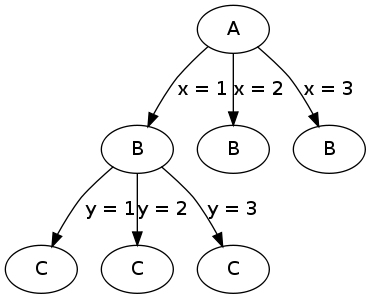
\includegraphics[scale=0.35]{controlflowanalysis.png}
    \end{column}
  \end{columns}
\end{frame}

\subsection{Processor Behaviour Analysis}
\begin{frame}{Processor Behaviour Analysis}
  \begin{itemize}
    \item Uses a model of the processor to determine the behaviour for each task
    \item Context is Important
      \begin{itemize}
        \item Memory, Cache
        \item Pipelines, Branch Prediction
        \item<3-> Time Anomalies
          \begin{itemize}
            \item<3-> ie: Cache misses due to branch mis-predictions
          \end{itemize}
      \end{itemize}
      \item<2-> The obvious worst-case may not be the actual worst-case
  \end{itemize}
\end{frame}

\subsection{Bound Calculation}
\begin{frame}{Bound Calculation}  
  \begin{itemize}
    \item Combines individual tasks' timings to get overall $WCET_D$
      \pause
    \item Three main approaches:
      \begin{itemize}
        \item Path-Based Calculation
        \item Structure-Based Calculation
        \item Implicit Path Enumeration Technique (IPET)
      \end{itemize}
  \end{itemize}
\end{frame}

\begin{frame}{Example Input}
  \begin{columns}
    \begin{column}{0.25\textwidth}
      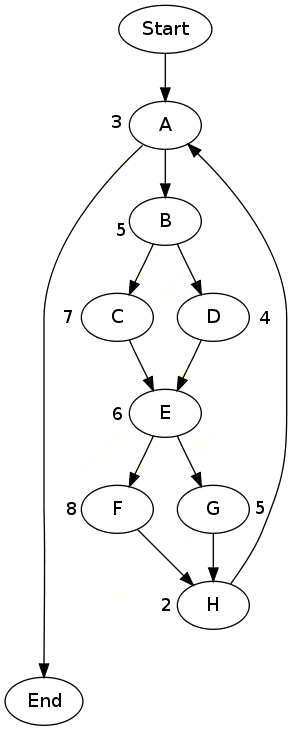
\includegraphics[scale=0.3]{input.png}
    \end{column}
    \begin{column}{0.75\textwidth}
      \begin{itemize}
        \item Nodes represent basic elements of the task
        \item Edges represent possible execution paths
        \item Values beside nodes indicate individual WCETs
        \item For the following examples: 100 loop iterations
      \end{itemize}
    \end{column}
  \end{columns}
\end{frame}

\begin{frame}{Structure-Based Bound Calculation}
  \begin{itemize}
    \item Bottom-up traversal of the syntax tree
    \item A set of rules is given for combining child nodes with parents
      \begin{itemize}
        \item Combine all possibilities of a conditional
        \item Combine sequential nodes
        \item Etc.
      \end{itemize}
    \item $T_{Parent} = WCET_{max}(T_{Child0}, T_{Child1},\dots)$
    \item Simple and computational cheap
    \item Inter-node dependencies or optimized code may cause problems
  \end{itemize}
\end{frame}

\begin{frame}{Structure-Based Bound Calculation Example}
  \begin{columns}
    \begin{column}{0.25\textwidth}
      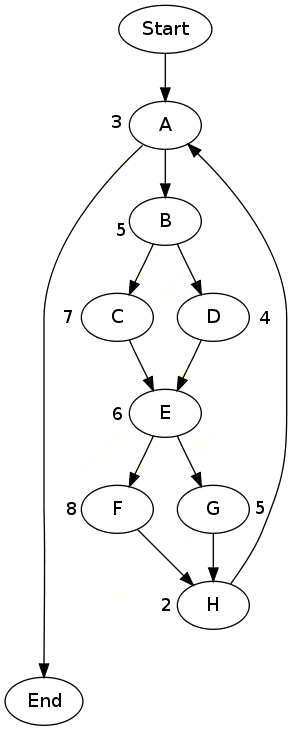
\includegraphics[scale=0.3]{structureoutput1.png}
    \end{column}
    \begin{column}{0.25\textwidth}
      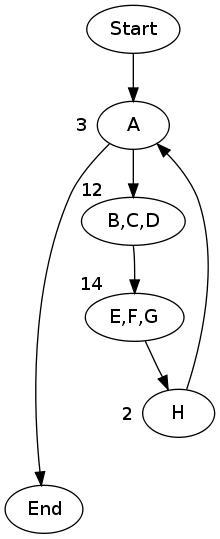
\includegraphics[scale=0.3]{structureoutput2.png}
    \end{column}
    \begin{column}{0.25\textwidth}
      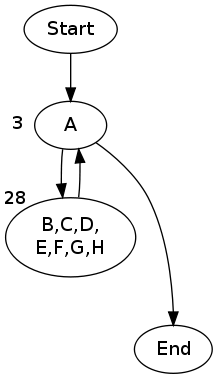
\includegraphics[scale=0.3]{structureoutput3.png}
    \end{column}
    \begin{column}{0.25\textwidth}
      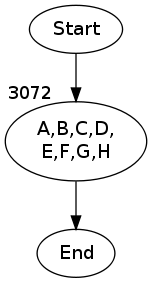
\includegraphics[scale=0.3]{structureoutput4.png}
    \end{column}
  \end{columns}
\end{frame}

\begin{frame}{Path-Based Bound Calculation}  
    \begin{columns}
    \begin{column}{0.25\textwidth}
      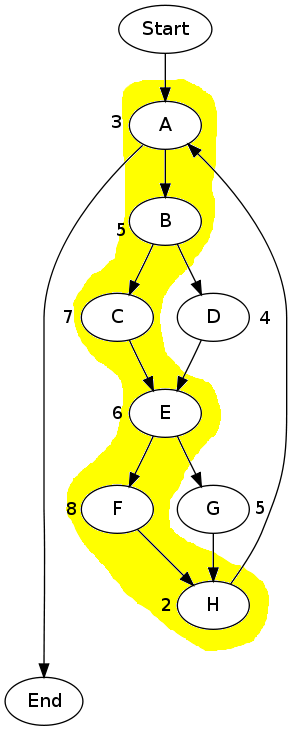
\includegraphics[scale=0.3]{pathoutput.png}
    \end{column}
    \begin{column}{0.75\textwidth}
      \begin{itemize}
        \item Each possible path is traversed, and $WCET_{PATHi}$ is calculated
        \item $WCET_D = max(WCET_{PATH0},WCET_{PATH1},\dots)$
          \pause
        \item Longest execution path is explicitly shown.
          \begin{itemize}
            \item Best target for optimizations
          \end{itemize}
        \item Analysis time rises exponentially with the number of branches
      \end{itemize}
    \end{column}
  \end{columns}
\end{frame}

\begin{frame}[IPET]{Implicit Path Enumeration Technique}
  \begin{itemize}
    \item Each node is assigned a time value, $t$, and a counter variable, $x$
    \item Program structure is represented as constraining linear equations
    \item $WCET_D$ can be found using either:
      \begin{itemize}
      \item Integer Linear Programming
        \begin{itemize}
          \item More popular method
          \item Efficient solvers exist
        \end{itemize}
      \item Constrain Satisfaction
        \begin{itemize}
          \item Allows for constraints that are more complex
          \item Generally slower than integer linear programming
        \end{itemize}
      \item In either case, the problem is NP-hard
      \end{itemize}
  \end{itemize}
\end{frame}

\begin{frame}{IPET Example}
  \begin{columns}
    \begin{column}{0.25\textwidth}
      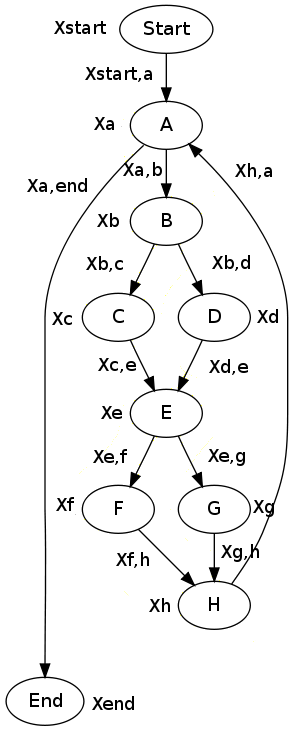
\includegraphics[scale=0.3]{ipetoutput.png}
    \end{column}
    \begin{column}{0.75\textwidth}
      \begin{eqnarray*}
        x_{start} &=& 1 \\
        x_{end} &=& 1 \\
        x_A &\leq& 100 \\
        x_A &=& x_{start,A} + x_{H,A} = x_{A,end} + x_{A,B} \\
        x_B &=& x_{A,B} = x_{B,C} + x_{B,D} \\
        x_C &=& x_{B,C} = x_{C,E} \\
        &\dots& \\
        x_H &=& x_{F,H} + x_{G,H} = x_{H,A} \\
        x_{end} &=& x_{A,end} \\
        WCET_D &=& maximize(\sum x_it_i)
      \end{eqnarray*}
    \end{column}
  \end{columns}
\end{frame}

\section{Measurement}
\subsection{}
\begin{frame}{Measurement}
  \begin{itemize}
    \item Results gathered experimentally by executing the task
    \item Infeasible to measure all possible cases of execution
    \item Provides an estimate of the WCET
    \item Generally not safe for hard real-time purposes
  \end{itemize}
\end{frame}

\end{document}
